\documentclass[aps,prd,twocolumn,showpacs,superscriptaddress,groupedaddress,nofootinbib]{revtex4}  % for review and submission
%\documentclass[aps,preprint,showpacs,superscriptaddress,groupedaddress]{revtex4}  % for double-spaced preprint
\usepackage{graphicx}  % needed for figures
\usepackage{dcolumn}   % needed for some tables
\usepackage{bm}        % for math
\usepackage{amsmath,amssymb}   % for math
\usepackage{aas_macros}
\usepackage{multirow}
\usepackage{color}
\usepackage{verbatim}
%\usepackage{times}
\usepackage{url}
\usepackage{hyperref}

% avoids incorrect hyphenation, added Nov/08 by SSR
\hyphenation{ALPGEN}
\hyphenation{EVTGEN}
\hyphenation{PYTHIA}

\newcommand{\mr}{\mathrm}
\newcommand{\tcb}{\textcolor{blue}}
\newcommand{\bea}{\begin{eqnarray}}
\newcommand{\eea}{\end{eqnarray}}
\newcommand{\bmp}{\bm{\Psi}}
\newcommand{\bms}{\bm{s}}
\newcommand{\bmk}{\bm{k}}
\newcommand{\bmx}{\bm{x}}
\newcommand{\bmq}{\bm{q}}
\newcommand{\la}{\langle}
\newcommand{\ra}{\rangle}

\begin{document}
% The following information is for internal review, please remove them for submission
\widetext
% the following line is for submission, including submission to the arXiv!!
%\hspace{5.2in} \mbox{Fermilab-Pub-04/xxx-E}

\title{Nonlinear Reconstruction}
%\title{Reconstruction beyond the Zel'dovich approximation}
%\title{Moving mesh reconstruction} 

\author{Hong-Ming Zhu}
\affiliation{Key Laboratory for Computational Astrophysics, National Astronomical Observatories, Chinese Academy of Sciences, 20A Datun Road, Beijing 100012, China}
\affiliation{University of Chinese Academy of Sciences, Beijing 100049, China}

\author{Yu Yu}
\affiliation{Key Laboratory for Research in Galaxies and Cosmology,
Shanghai Astronomical Observatory, Chinese Academy of Sciences,
80 Nandan Road, Shanghai 200030, China}

\author{Ue-Li Pen}
\affiliation{Canadian Institute for Theoretical Astrophysics, University of Toronto, 60 St. George Street, Toronto, Ontario M5S 3H8, Canada}
\affiliation{Dunlap Institute for Astronomy and Astrophysics, University of Toronto, 50 St. George Street, Toronto, Ontario M5S 3H4, Canada}
\affiliation{Canadian Institute for Advanced Research, CIFAR Program in Gravitation and Cosmology, Toronto, Ontario M5G 1Z8, Canada}
\affiliation{Perimeter Institute for Theoretical Physics, 31 Caroline Street North, Waterloo, Ontario, N2L 2Y5, Canada}

\author{Xuelei Chen}
\affiliation{Key Laboratory for Computational Astrophysics, National Astronomical Observatories, Chinese Academy of Sciences, 20A Datun Road, Beijing 100012, China}
\affiliation{University of Chinese Academy of Sciences, Beijing 100049, China}
\affiliation{Center of High Energy Physics, Peking University, Beijing 100871, China}

\author{Hao-Ran Yu}
\affiliation{Kavli Institute for Astronomy and Astrophysics, Peking University, Beijing 100871, China}
\affiliation{Canadian Institute for Theoretical Astrophysics, University of Toronto, 60 St. George Street, Toronto, Ontario M5S 3H8, Canada}


\date{\today}

\begin{abstract}
We present a new method to reconstruct the primordial (linear) density field
using the estimated nonlinear displacement field. The divergence of 
the displacement field gives the reconstructed density field. We solve the 
nonlinear displacement field ... ... 
\end{abstract}

\pacs{}
\maketitle

%\section{\label{sec:level1}First-level heading}
% sections are not used for PRL papers

{\it Introduction.}---

Observations of cosmological large scale structure is a cornerstone in
modern cosmology.  Ambitious surveys are mapping large swaths of the
visible universe (CHIME, Tianlai, DESI, PFS, etc).  Precision
measurements of baryon acoustic oscillations, RSD, FNL, etc, are
continually improving.  The precision of the measurement is often
limited by strong non-Gaussianity of the dark matter and galaxy
density fields on small scales, which prevent a simple mapping to the
initial conditions that are predicted by cosmological theories.  The
%loss of coherence to the initial conditions has been known as
mode-mode coupling, information saturation, etc.

Some of the couplings are understood as arising from the coupling of
large scale linear modes to smaller scale still linear modes
(e.g. Tides, Supersample variance).  These can be corrected by a
linear mapping, also known as 'reconstruction' (cite Seo, Padmanabhan,
etc).

Recent work showed that the $z=0$ Lagrangian space non-linear
displacement potential correlates with the initial linear field (arxiv
1610.07112) to a $k\sim 2h$/Mpc, about an order of magnitude shorter
length scale than observed in Eulerian space.  That worked required
knowing the actual displacement of dark matter particles, which in
practice is not observable.  In this paper we implement the
combination of the mass ordering coordinate of 1609.07041 with the
E-mode displacement field, resulting in a unique solution that has a
comparable reconstruction fidelity as the true E-mode displacement field.

The observed large-scale structure provides ...
In this Letter, we solve the nonlinear displecement field from the nonlinear 
density field and present a new method to reconstruct the primordial density
field and hence the linear BAO information.

The analysis usually uses the density field directly. measure the power spectrum
However, modeling the small-scale inhomogeneities limits to $k<0.1\ h/\mr{Mpc}$.
We find the nonlinearities in the displacement field is much more linear than 
the density field. The correlation of the divergence of the displacement field
with the primordial (linear) density field is much better than that of the 
nonlinear density field. The divergence of the reconstructed nonlinear
displacement gives the reconstructed density field, which is much more linear
than the nonlinear density field.

%=========

{\it Displacement decomposition.}---In the Lagrangian picture of structure 
formation, 
the displacement field $\bm{s}(\bm{q},\tau)$ fully describes the motion of each mass element. The Eulerian position $\bm{x}$ of a mass element is given by
\bea
\bm{x}(\bm{q},\tau)=\bm{q}+\bm{s}(\bm{q},\tau),
\eea
where $\bm{q}$ is the initial Lagrangian position of this mass element.
The displacement field $\bm{s}(\bm{q})$ can be decomposed into a gradient part
and a curl part,
\bea
\bm{s}(\bm{q})=\bm{s}_E(\bm{q})+\bm{s}_B(\bm{q}),
\eea
where $\nabla\times\bm{s}_E=0$ and $\nabla\cdot\bm{s}_B=0$.
The gradient part can be completely described by a scalar potential,
while the curl part has two independent components.

In the 1D cosmology, the displacement field has only one component though 
it is a vector field \cite{2016matt}. 
This allows us to determine the displacement field 
from the density field, which is a scalar field \cite{2016arXiv160907041Z}.
However, the motion has three degrees of freedom in 3D instead of one.
Since from cosmological observations we only have the density field, we expect 
to reconstruct the scalar part of the displacement field.

%=========

{\it Reconstruction algorithm.}---The basic idea is to build a curvilinear 
coordinate system $\bm{\xi}\equiv(\xi_1,\ \xi_2,\ \xi_3)$, where the mass per
volume element is constant. 
In order to determine the physical position of each lattice point, we need to 
specify the Cartesian coordinate $\bm{x}(\bm{\xi},\ t)$ of each curvilinear 
coordinate.
Since we attemp to follow the potential flow instead of the vorticity, we 
define a coordinate transformation that is a pure gradient,
\bea
\label{eq:trs}
x^i=\xi^\mu\delta^i_\mu+\Delta x^i,
\eea
where
\bea
\Delta x^i\equiv\frac{\partial\phi}{\partial\xi^\nu}\delta^{i\nu}.
\eea
Here, $\Delta{x}^i$ is the {\it lattice displacement} and $\phi$ the 
{\it deformation potential} \cite{1995ApJS..100..269P,1998ApJS..115...19P}. 
The new coordinate frame gives the estimated initial Lagrangian coordinates. 
The difference between these two frames is the estimated nonlinear displacement.
Here, Latin indices denote Cartesian coordinate labels $x^i$, while Greek 
indices denote the curvilinear coordinates $\xi^\alpha$.

There are many possible ways to determine the new coordinate frame. 
One efficient and robust algorithm is the moving grid approach \cite{1995ApJS..100..269P,1998ApJS..115...19P}.
This approach is originally introduced for the adaptive particle-mesh $N$-body 
code \cite{1995ApJS..100..269P} and the moving mesh hydrodynamics code
\cite{1998ApJS..115...19P}. 
The moving grid based simulation algorithm adopts a curvilinear moving grid
which evolves towards a state of constant mass per grid cell. 
The evolution of the deformation potential is determined by a linear elliptic
evolution equation
\bea
\label{eq:pde}
\partial_\mu(\rho\sqrt{g}e^\mu_i\delta^{i\nu}\partial_\nu\dot{\phi})=\Delta\rho,
\eea
where $e^\mu_i$ is the matrix inverse of the triad $e^i_\mu=\partial x^i/\partial\xi^\mu$, $\sqrt{g}=\mr{det}(\partial x^i/\partial \xi^\alpha)$ and 
$\Delta\rho=\bar{\rho}-\rho\sqrt{g}$. 
See Ref. \cite{1995ApJS..100..269P} for a simple physical intepretation of 
Eq. (\ref{eq:pde}).
The ellpitic equation can be solved using the multigrid algorithm described 
in Ref. \cite{1995ApJS..100..269P}.

Since the displacement from the initial Lagrangian coordinate to the final 
Eulerian coordinate can be large, the elliptic equation must then be solved 
iteratively. We obtain the change of the deformation potential 
$\Delta\phi=\dot{\phi}\Delta t$ at each time step and then update the density
field in the new Cartesian coordinate frame.  
The solution is given by 
\bea
\phi=\Delta\phi^{(1)}+\Delta\phi^{(2)}+\Delta\phi^{(3)}+\cdots
\eea
where $\Delta\phi^{(i)}$ is the result from the $i$th iteration. 
We also implement the smoothing and limiting schemes to guarantee the triad 
$e^\mu_i$ is positive definite \cite{1995ApJS..100..269P,1998ApJS..115...19P},
from which we have the relation $\partial x^a/\partial\xi^a>0$ (no summation).
From this equality, it follows that each Cartesian coordinate increases monotonically as a function of its corresponding curvilinear coordinate.
Then, the negative divergence of the estimated displacement gives the 
reconstructed density field 
\bea
\delta_r(\bm{\xi})=-\nabla_{\bm{\xi}}\cdot\Delta\bm{x}(\bm{\xi})
=-\nabla^2_{\bm{\xi}}\phi(\bm{\xi}).
\eea
where $\bm{\xi}$ is the estimated initial Lagrangian coordinate.
In the case that particles follow a irrotational potential flow and no shell
crossing happens, the reconstructed displacement is exact up to a global 
spatial translation.
However, shell crossing happens in the nonlinear regime. This reconstruction
algorithm gives an effective displacement.
%=======================================


{\it Implementation and results.}---To test the performance of 
the new reconstruction algorithm, we run $N$-body simulations with 
the $\mr{CUBEP}^3\mr{M}$ code \cite{2013code}.
The simulation involves $2048^3$ dark matter particles in a box of 
side length $600\ \mr{Mpc}/h$.
In the analysis, we use the output at $z=0$. Mass densities are computed
on $512^3$ grids. 
The nonlinear reconstruction code is based on the {\tt CALDEFP} subroutine from 
the moving mesh hydrodynamics code \cite{1998ApJS..115...19P}.
The nonilnear reconstruction code solves the deformation potential iteratively.
We test convergence by comparing results from different time steps and 
find the reconstrution converges after 1500 time steps for the nonlinear 
density field on $512^3$ grids. 
We also scale the initial density field at $z=100$ by the linear growth factor
to get the linear density field at $z=0$.

\begin{figure}[tbp]
\begin{center}
\includegraphics[width=0.48\textwidth]{map0512-0128_i1500_.eps}
\end{center}
\vspace{-0.7cm}
\caption{The nonlinear density field at $z=0$ and the projected deformed grid 
from reconstruction. The grid lines show good correlation with the density 
field.}
\label{fig:den}
\end{figure}

Figure \ref{fig:den} shows a slice of the nonlinear density field. 
We also overplot the deformed grid on the density field. The grid becomes 
denser in the higher density region and sparser in the lower density region.
The grid lines also show strong correlation with the filementary structures.
The difference between the regular grid and the deformed grid is the estimated
displacement field, whose divergence gives the reconstructed linear density 
field. The nonlinear density field $\delta(\bm{x})$ is given on the Eulerian 
position $\bm{x}$, while the reconstructed density field $\delta_r(\bm{\xi})$ 
is computed on the estimated Lagrangian position $\bm{\xi}$. Due to the 
limiting and smoothing schemes we use, the grid never overlaps itself as in 
Refs. \cite{1995ApJS..100..269P,1998ApJS..115...19P}.

To conveniently quantify the linear information $\delta_L$ in the reconstructed
density field $\delta_r$, we decompose the reconstruted field $\delta_r$ as
\bea
\delta_r(k)=b_r(k)\delta_L(k)+n_r(k),
\eea
where $b_r(k)=P_{\delta_r\delta_L}(k)/P_{\delta_L}(k)$. 
Here, $b_r\delta_L$ is completely correlated with the linear density field 
$\delta_L$ and $n_r$ uncorrelated with the linear density field $\delta_L$.
The power spectrum of the reconstructed field can be written as
\bea
P_{\delta_r}(k)=b_r^2(k)P_{\delta_L}(k)+P_{n_r}(k),
\eea
where $b_r^2$ is the nonlinear damping factor. 
For the nonlinear density field, we also have
\bea
P_{\delta}(k)=b^2(k)P_{\delta_L}(k)+P_{n}(k),
\eea
where $b(k)=P_{\delta\delta_L}(k)/P_{\delta_L}(k)$. 
In Fig. \ref{fig:ps}, we plot the linear components and the noise terms of the
nonlinear and reconstructed fields. The noise part dominates over the linear 
signal at $k\gtrsim0.6\ \mr{Mpc}/h$, indicating that all BAO peaks can be 
measured to an unprecented accuracy.

\begin{figure}[tbp]
\begin{center}
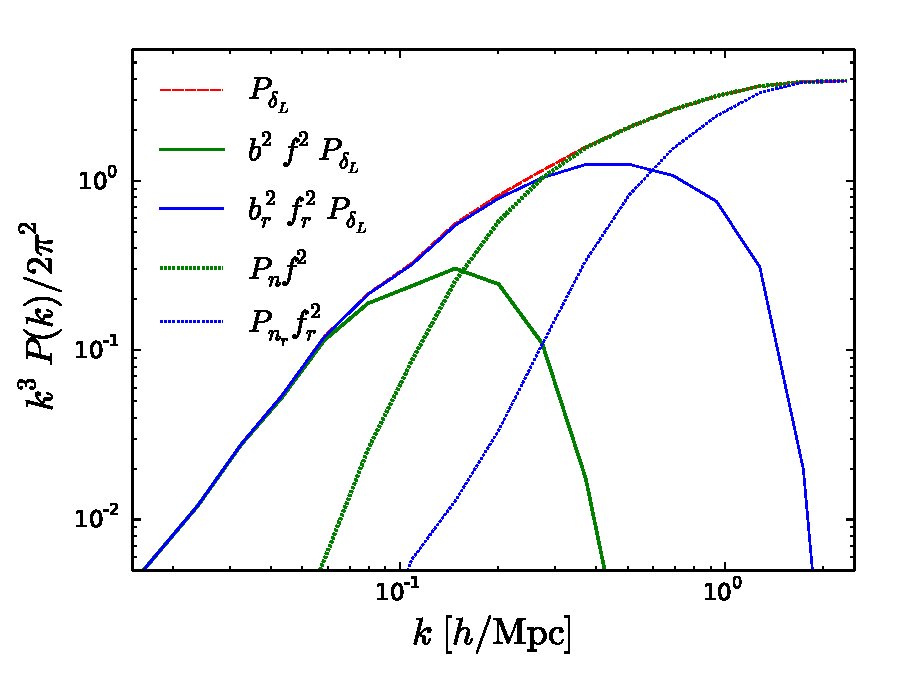
\includegraphics[width=0.48\textwidth]{fb.eps}
\end{center}
\vspace{-0.7cm}
\caption{The linear power spectrum (dashed line), the linear parts of the
nonlinear (thick solid line) and reconstructed (thin solid line) power spectra,
the noise parts of the nonlinear (thick dotted line) and reconstructed
(thin dotted line) power spectra.
For visual comparisions, we rescale both the linear and noise parts by
$f^2=P_{\delta_L}/P_{\delta}$ and $f^2_r=P_{\delta_L}/P_{\delta_r}$ for the nonlinear and reconstructed fields, respectively.
The noise terms dominate over the signals at
$k\gtrsim0.1\ \mr{Mpc}^{-1}$ for the nonlinear field and $k\gtrsim0.6\ \mr{Mpc}^{-1}$
for the reconstructed field.}
\label{fig:ps}
\end{figure}

Reconstruction reduces the nonlinear damping $b^2(k)$ as well as the
noise term $P_{n}(k)$. To quantify the overall performance, we can use the
cross-correlation coefficient
\bea
r(k)=\frac{P_{\delta\delta_L}(k)}
{\sqrt{P_{\delta}(k)P_{\delta_L}(k)}}
=\frac{1}{\sqrt{1+\eta(k)}},
\eea
where $\eta=P_n/(b^2P_{\delta_L})$ quantifies the relative amplitude
of $n$ with respect to $b\delta_L$. 
In Fig. \ref{fig:xcc}, we plot the cross-correlation coefficients.
The correlation of the reconstructed field $\delta_r$ with the linear density
field $\delta_L$ is almost the same as that of the nonlinear density field 
$\delta$ at $z=5$, which is better than the 1D case, where the correlation of
$\delta_r$ with $\delta_L$ is only comparable to that of $\delta$ 
at $z=3$ \cite{2016arXiv160907041Z}.
This is also as expected since the nonlinear evolution in 1D is more
significant than the 3D case \cite{2016matt}.
We also show the cross-correlation coefficient of $\delta_E$ with $\delta_L$,
where $\delta_E(\bm{q})=-\nabla\cdot \bm{s}_E(\bm{q})$ is the negative 
divergence of the real displacement from simulation.
It is still hard to recover linear modes at $k\gtrsim1h/\mr{Mpc}$, since some information has been irreversibly lost in nonlinear evolution. 


\begin{figure}[tbp]
\begin{center}
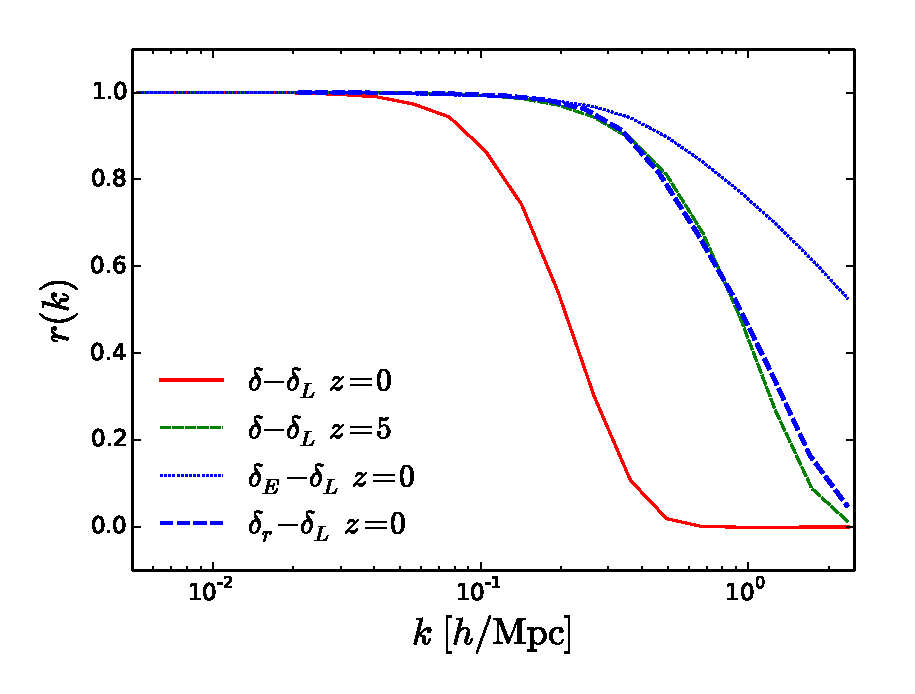
\includegraphics[width=0.48\textwidth]{fa.eps}
\end{center}
\vspace{-0.7cm}
\caption{
The $\delta-\delta_L$ correlation coefficients at $z=0$ (solid
line) and $z=5$ (thin-dashed line), the $\delta_E-\delta_L$ correlation
coefficient (dotted line), as well as the $\delta_r-\delta_L$
correlation coefficient (thick-dashed line).}
    
\label{fig:xcc}
\end{figure}

The density fluctuation probability distribution function (PDF) quantifies 
the Gaussianity of the density field. 
Figure \ref{fig:pdf} shows the PDFs of the density fields. 
Since the PDFs depend on the grid scale, we apply the Wiener filter
\bea
W(k)=\frac{P_{\delta_L}(k)}{P_{\delta_L}(k)+P_{n_r}(k)/b_r^2(k)}
\eea
to both the reconstructed and linear fields to get the converged results.
The reconstructed density field is well correlated with the linear density 
field and also much more Gaussian than the original nonlinear density field.
The new reconstruction method are expected to reduce the correlation in the 
covariance matrix and increase the information content of the power spectrum
\cite{1999MNRAS.308.1179M,1999ApJ...527....1S,2005MNRAS.360L..82R}.
Notice that the values of the reconstructed density field $\delta_r$ are always
smaller than 3. 
The compression limiter constrains $\partial x^a/\partial\xi^a\geq0.1$ 
\cite{1995ApJS..100..269P,1998ApJS..115...19P}.
The reconstructed density field is given by the negative
divergence of the estimated nonlinear displacement field
$\delta_r=-\nabla\cdot\Delta{\bm{x}}=3-\nabla\cdot\bm{x}$,
where $\nabla\cdot\bm{x}=\partial x^1/\partial\xi^1+\partial x^2/\partial\xi^2
+\partial x^3/\partial\xi^3$. 
We find the maximum value is $2.7$ for the reconstructed density field.  
This has confirmed that we have a continuous sequence of 
nondegenerate triads in the reconstruction. 
In the 1D case, the maximum value is 1 since we only have one spatial dimension
in the 1D cosmology \cite{2016arXiv160907041Z}.


\begin{figure}[tbp]
\begin{center}
\includegraphics[width=0.48\textwidth]{pdfwf-b.eps}
\end{center}
\vspace{-0.7cm}
\caption{The joint probability distribution function of the reconstructed field 
    $\delta_r$ and linear density field $\delta_L$. We also plot the 
probability distrbution functions of $\delta_r$ and $\delta_L$. Both fields
have been Wiener filtered to get converged results. The value of the 
reconstructed density field is always smaller than 3.}
\label{fig:pdf}
\end{figure}

{\it Discussions.}---The new reconstruction method reduces the nonlinearities 
significantly and successfully recovers a lot of linear modes 
at $k<0.6\ h/\mr{Mpc}$, which is about all the linear BAO information.
This has significant implications for measuring BAO in the current and future 
surveys, especially for volume-limited galaxy samples. 
To apply the new reconstruction method to observations, we need to consider 
reconstruction from galaxy density fields with redshift space distortions.
The modelling of the reconstructed density field will also be simplified since
less nonlinear effects are involved in the current method.
We intend to investigate these in subsequent works. 

The new method is also useful for improving the measurement of redshift space
distortions. The nonlinear displacement is much more linear than
the nonlinear density field. 
This also simplifies the modelling of RSD, which is usually
limited by nonlinearities \cite{2013PhRvD..87f3526Z}.
The current method to reconstruct velocity field from the observed density 
fieldis derived from the linearized continuity equation. 
The nonlinear density field is usually smoothed on the linear scale
($\sim10\ \mr{Mpc}/h$) to make the linear approximation valid.
We can also reconstruct the velocity field from the estimated displacement 
field.
This requires a detailed study of the correlation between the displacement 
field and the velocity field, which will be presented in future.

Neutrinos are expect to suppress the growth of structure on scales below the 
neutrino thermal free-streaming scale \cite{1980bond,1997hu}.
It is interesting to study the effect of neutrinos on the Lagrangian space 
clustering. 
The new method is also crucial for measuring the dark matter-neutrino cross 
correlation dipole \cite{2014zhm,2016zhm}. 


ELUCID \cite{2014ApJ...794...94W}?
The reconstructed nonlinear displacement can be further improved ...?
%=======================================


The simulations were performed on the BGQ supercomputer at the SciNet HPC 
Consortium. SciNet is funded by the Canada Foundation for Innovation under 
the auspices of Compute Canada, the Government of Ontario, the Ontario Research 
Fund Research Excellence, and the University of Toronto.
We acknowledge the support of the Chinese MoST 863 program under Grant 
No. 2012AA121701, the CAS Science Strategic Priority Research Program 
XDB09000000, the NSFC under Grant No. 11373030, IAS at Tsinghua University, 
 and NSERC.
The Dunlap Institute is funded through an endowment established by the David Dunlap family and the University of Toronto.
Research at the Perimeter Institute is supported by the Government of Canada
through Industry Canada and by the Province of Ontario through the Ministry of
Research $\&$ Innovation.

\bibliographystyle{apsrev}
\bibliography{3d}

\end{document}
